\documentclass[10pt,a4paper]{article}
\usepackage[margin=1.8cm]{geometry}
\usepackage[T1]{fontenc}
\usepackage{lmodern,amsmath,amssymb,booktabs,graphicx,caption,enumitem}
\usepackage{newunicodechar}
\usepackage[hidelinks]{hyperref}
\graphicspath{{../figures/}}
\captionsetup{font=small,labelfont=bf}
\setlist{nosep,leftmargin=*}
\setlength{\parskip}{3pt}
\newunicodechar{≈}{\ensuremath{\approx}}
\newunicodechar{≪}{\ensuremath{\ll}}
\newunicodechar{→}{\ensuremath{\to}}
\newunicodechar{×}{\ensuremath{\times}}
\newunicodechar{∝}{\ensuremath{\propto}}
\newunicodechar{ε}{\ensuremath{\varepsilon}}
\newunicodechar{≥}{\ensuremath{\geq}}
\newunicodechar{≤}{\ensuremath{\leq}}
\newunicodechar{√}{\ensuremath{\surd}}
\newunicodechar{μ}{\ensuremath{\mu}}
\newunicodechar{−}{\ensuremath{-}}
\newunicodechar{·}{\ensuremath{\cdot}}
\title{\vspace{-1.4cm}Exploring the Roofline Model: matrix–vector vs. matrix–matrix multiplication\vspace{-0.3cm}}
\author{Scientific Programming and Large Scale Computing — Homework 4 \\ \small Aldana Montagut Barri}
\date{\vspace{-0.6cm}}
\begin{document}
\maketitle

\section{Implementation and methodology}
Both operations are implemented in NumPy (\texttt{kernels.py}): matrix–vector multiplication \textbf{y} = \textbf{A} \textbf{x} and matrix–matrix multiplication \textbf{C} = \textbf{A} \textbf{B} are computed with \texttt{np.matmul}, writing into a pre-allocated \texttt{out=} array. NumPy passes them to the BLAS routines GEMV and GEMM of OpenBLAS 0.3.34. The operands are initialised with constants (\texttt{A=1}, \texttt{B=2}, \texttt{x=3}) and the outputs are allocated beforehand, so neither allocation nor initialisation is timed. For every size \emph{N} and precision, \texttt{benchmark.py} performs two untimed warm-up calls and then times calls with \texttt{time.perf\_counter} until at least 5 repetitions and 0.5 s of work have been collected; the median is reported. float32 and float64 are run back-to-back for each \emph{N}, so that both see the same machine state. Every result is checked against the exact value (\emph{y}\textsubscript{i} = 3\emph{N}, \emph{C}\textsubscript{ij} = 2\emph{N}) with a tolerance-based comparison; all checks passed. The sweep covers \emph{N} = 128–16384 (matrix–vector) and \emph{N} = 64–4096 (matrix–matrix) in steps of about √2, once with one BLAS thread and once with all threads, back-to-back on 14 Nov 2026.

\textbf{Two runs, two roles.} The single-thread run is the main evidence for the scaling and for the cache-versus-main-memory behaviour: one core, no thread start-up cost and the smallest run-to-run spread. The all-threads run is used for the peak performance and the Roofline plots. Every number below states which run it comes from.

\textbf{Machine.} Dell Latitude 7490 on mains power: Intel Core i7-8650U (4 cores/8 threads, 1.9 GHz base, up to 4.2 GHz turbo, 15 W TDP, AVX2 with two FMA units per core), dual-channel DDR4-2400, Windows 11, Python 3.14, NumPy 2.5. In this report \textbf{cache} means the 8 MB last-level (L3) cache shared by the four cores, and \textbf{main memory} means the DDR4 memory behind it. A problem \emph{fits in cache} when its whole working set (\textbf{A}, \textbf{x} and \textbf{y}) is at most 8 MB.

\emph{Theoretical roofline.} \emph{P}\textsubscript{peak} = 4 cores × \emph{f} × 16 (float64) or 32 (float32) FLOP/cycle. The clock \emph{f} is not fixed: it moves between the 1.9 GHz base and the 4.2 GHz maximum turbo depending on power, temperature and load, so the compute ceiling is a band: 121.6–268.8 GFLOP/s (float64) and 243.2–537.6 GFLOP/s (float32). \emph{B}\textsubscript{mem} = 2 channels × 8 B × 2.4 GT/s = 38.4 GB/s. The ridge points \emph{I}\textsubscript{ridge} = \emph{P}\textsubscript{peak}/\emph{B}\textsubscript{mem} are 3.2–7.0 (float64) and 6.3–14.0 (float32) FLOP/byte. \emph{Measured ceilings.} A bandwidth probe that copies 256 MB arrays reaches 20.5 GB/s, and the best matrix–matrix calls (all threads) reach 99.4 (float64) and 202.4 GFLOP/s (float32).

\section{Theoretical arithmetic intensity}
Let \emph{s} be the size of one element (\emph{s} = 4 B for float32, 8 B for float64). Each output entry is a dot product of length \emph{N}: \emph{N} multiplications and \emph{N} − 1 additions, i.e. ≈ 2\emph{N} FLOP (a fused multiply–add counts as two). The traffic estimate assumes perfect reuse: every array moves between main memory and the processor exactly once (the \emph{compulsory} traffic).

\begin{itemize}
\item \textbf{Matrix–vector}: \emph{F} = 2\emph{N}\textsuperscript{2}; \emph{Q} = (\emph{N}\textsuperscript{2} + 2\emph{N})·\emph{s} (read \textbf{A} and \textbf{x}, write \textbf{y}); \emph{I} = \emph{F}/\emph{Q} → 2/\emph{s}. Every element of \textbf{A} is used only once, so no reuse can improve this: \textbf{A} dominates the traffic and \emph{I} is fixed at 0.25 (float64) or 0.5 (float32) FLOP/byte, independent of \emph{N}. Only \textbf{x} (a few kB, it stays in cache) is reused. If even \textbf{x} were re-read for every row, \emph{Q} ≈ 2\emph{N}\textsuperscript{2}\emph{s} and \emph{I} ≈ 1/\emph{s}.
\item \textbf{Matrix–matrix}: \emph{F} = 2\emph{N}\textsuperscript{3}; \emph{Q} = 3\emph{N}\textsuperscript{2}\emph{s} (read \textbf{A}, \textbf{B}, write \textbf{C}); \emph{I} = 2\emph{N}/(3\emph{s}), i.e. \emph{N}/12 (float64) and \emph{N}/6 (float32). Each element of \textbf{A} and \textbf{B} is used \emph{N} times, so \emph{I} grows with \emph{N}. This is an upper bound: it needs all three matrices to stay in cache. For \emph{N} = 4096 they occupy 400 MB (float64), so BLAS splits the matrices into cache-sized blocks of size \emph{b} and re-reads each block about \emph{N}/\emph{b} times, giving \emph{I} \textasciitilde{} \emph{b}/\emph{s}. With no reuse at all (both operands fetched for every multiply–add) \emph{I} would fall to ≈ 1/\emph{s}, the same as matrix–vector.
\end{itemize}
\begin{table}[h]\centering\small
\begin{tabular}{lccccc}\toprule
 & FLOP & bytes (compulsory) & \emph{I} float32 & \emph{I} float64 & \emph{I} at \emph{N} = 4096 (float32 / float64) \\\midrule
Matrix–vector \textbf{y} = \textbf{A} \textbf{x} & 2\emph{N}\textsuperscript{2} & (\emph{N}\textsuperscript{2} + 2\emph{N})·\emph{s} & → 0.5 & → 0.25 & 0.50 / 0.25 \\
Matrix–matrix \textbf{C} = \textbf{A} \textbf{B} & 2\emph{N}\textsuperscript{3} & 3\emph{N}\textsuperscript{2}·\emph{s} & \emph{N}/6 & \emph{N}/12 & 683 / 341 \\
\bottomrule\end{tabular}
\caption{Theoretical FLOP count, compulsory memory traffic and arithmetic intensity (FLOP/byte).}
\end{table}

Compared with the ridge points, matrix–vector multiplication (\emph{I} = 0.25–0.5 ≪ 3.2–14) is \emph{memory-bound} for every \emph{N}: its ceiling is \emph{B}·\emph{I}, i.e. 9.6 (float64) / 19.2 GFLOP/s (float32) with the theoretical bandwidth and 5.1 / 10.3 GFLOP/s with the measured 20.5 GB/s. Matrix–matrix multiplication crosses the ridge at \emph{N} ≈ 38 (base clock) to 84 (maximum turbo), and is therefore \emph{compute-bound} for practically all tested sizes. Halving \emph{s} doubles \emph{I} for both operations and doubles \emph{P}\textsubscript{peak} (twice as many values per AVX register), so the ideal float32 speed-up is 2× in both regimes.

\section{Results}
\begin{figure}[h]\centering
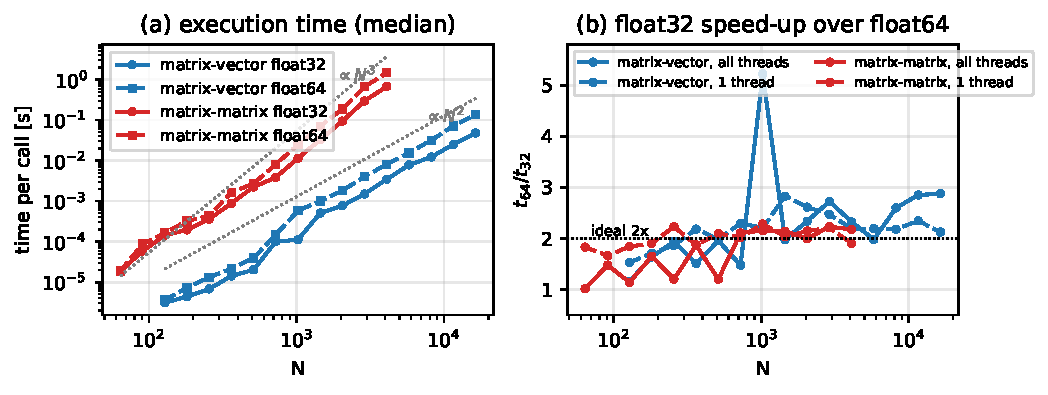
\includegraphics[width=\textwidth]{fig1_time_speedup.pdf}\vspace{-2mm}
\caption{(a) Median time per call, all threads; dotted lines show \emph{N}\textsuperscript{2} and \emph{N}\textsuperscript{3}. (b) Ratio \emph{t}\textsubscript{float64}/\emph{t}\textsubscript{float32} (solid: all threads, dashed: one thread).}
\end{figure}

\begin{figure}[h]\centering
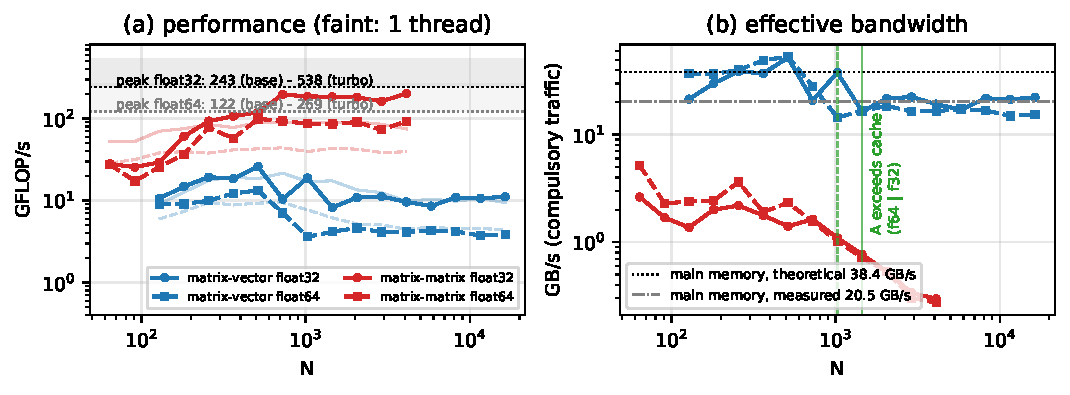
\includegraphics[width=\textwidth]{fig2_perf_bandwidth.pdf}\vspace{-2mm}
\caption{(a) Achieved GFLOP/s, all threads (faint lines: one thread); the shaded bands are the compute ceilings between base clock and maximum turbo. (b) Effective bandwidth computed from the compulsory traffic \emph{Q} (all threads); vertical lines mark where \textbf{A} no longer fits in the 8 MB cache (\emph{N} ≈ 1024 float64, 1448 float32).}
\end{figure}

\begin{table}[h]\centering\small
\begin{tabular}{p{7.4cm}cc}\toprule
 & 1 thread & all threads \\\midrule
Matrix–vector from cache, best bandwidth (float32 / float64) & 43.4 / 38.3 GB/s & 52.1 / 53.3 GB/s \\
Matrix–vector from main memory, \emph{N} ≥ 4096: bandwidth (float32 / float64) & 18.9–21.2 / 17.8–18.9 GB/s & 17.1–22.2 / 15.0–17.3 GB/s \\
Matrix–vector from main memory, \emph{N} ≥ 4096: performance (float32 / float64) & 9.5–10.6 / 4.5–4.7 GFLOP/s & 8.6–11.1 / 3.7–4.3 GFLOP/s \\
Matrix–matrix, saturated performance (float32 / float64) & 75–91 / 38–44 GFLOP/s & 163–202 / 73–99 GFLOP/s \\
Fitted exponent \emph{p} in \emph{t} ∝ \emph{N}\textsuperscript{p}: matrix–vector from main memory (float32 / float64) & 2.21 / 2.17 & 1.94 / 2.01 \\
Fitted exponent \emph{p}: matrix–matrix, \emph{N} ≥ 256 (float32 / float64) & 3.01 / 3.01 & 2.75 / 2.94 \\
\bottomrule\end{tabular}
\caption{Key measured values. Saturated matrix–matrix performance: \emph{N} ≥ 256 (1 thread), \emph{N} ≥ 724 / 512 (all threads, float32 / float64). Full tables: \texttt{results/tables.md}.}
\end{table}

\textbf{Matrix–vector} (Fig. 2, blue; Table 2). Two regimes appear. While the working set fits in cache, the effective bandwidth reaches 35–43 GB/s with one thread and up to 53 GB/s with all threads, i.e. above the theoretical main-memory bandwidth, which is possible because the data does not come from main memory. Once the matrix is larger than the cache, the bandwidth falls to a plateau of 18–21 GB/s (one thread): 49–55 \% of the theoretical 38.4 GB/s and close to the 20.5 GB/s of the bandwidth probe. The performance follows the bandwidth: about 10 GFLOP/s (float32) and 4.5 GFLOP/s (float64) with one thread, only about 4 \% of the base-clock peak. With one thread the transition is gradual rather than a single step: float64 falls from 9.4 GFLOP/s at \emph{N} = 724 (4 MB) to 7.7 (8 MB), 6.2 (16 MB), 5.2 (32 MB) and 4.5 GFLOP/s at 128 MB. Using all four cores does not help once the data is in main memory (speed-up 0.9–1.2× for \emph{N} ≥ 4096), because a single core already uses most of the available bandwidth.

\textbf{Matrix–matrix} (red). After a ramp-up for small \emph{N}, the performance saturates. With one thread it stays at 75–91 GFLOP/s (float32) and 38–44 GFLOP/s (float64) from \emph{N} = 256 upwards; with all threads at 163–202 GFLOP/s (float32) and 73–99 GFLOP/s (float64), i.e. 67–83 \% and 60–82 \% of the base-clock peak. Four cores give only 2.0–2.7× the single-core performance, not 4×, because the 15 W processor lowers its clock when all cores are busy. Unlike matrix–vector, matrix–matrix still gains from more cores, because it is limited by arithmetic and not by the shared memory bus. The bandwidth implied by the compulsory traffic falls as 1/\emph{N} (from about 5 to 0.3 GB/s, Fig. 2b), far below what main memory can deliver.

\begin{figure}[h]\centering
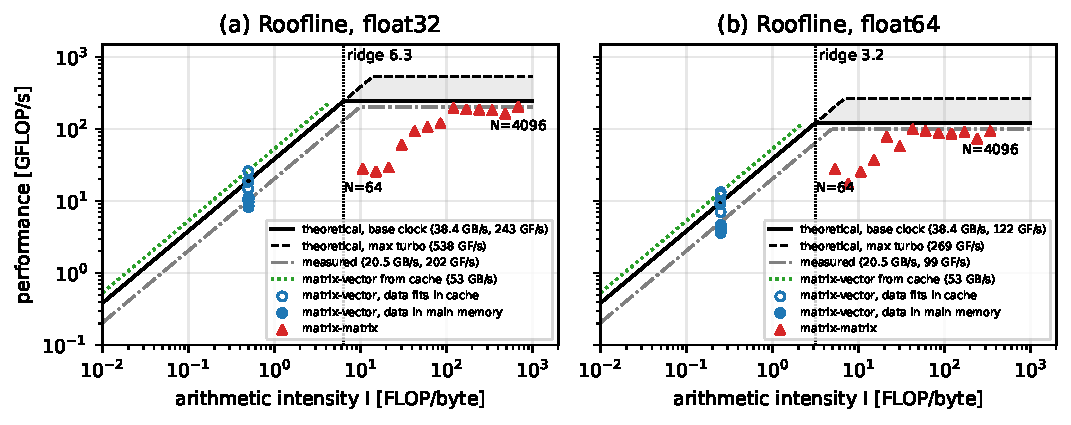
\includegraphics[width=\textwidth]{fig3_roofline.pdf}\vspace{-2mm}
\caption{Roofline plots (all threads) with the theoretical ceilings at base clock (solid) and maximum turbo (dashed, shaded band in between), the measured ceiling (dash-dot), and the bandwidth reached by matrix–vector from cache (dotted). The measurements are placed at their theoretical intensity. Hollow circles: data fits in cache.}
\end{figure}

\textbf{Roofline interpretation} (Fig. 3). Matrix–vector sits on the bandwidth slope, far left of the ridge. Its main-memory points (filled) lie close to the measured ceiling (some float32 points slightly above it, see Section 4), and its cache points (hollow) lie above the main-memory roof. This is expected: the actual intensity depends on the memory level considered, and when the data lives in cache the main-memory bandwidth is the wrong ceiling. Matrix–matrix sits right of the ridge and approaches the flat compute roof as \emph{N} grows. Small products (\emph{N} ≤ 128) lie well below both roofs: they are limited by fixed overheads (Python/NumPy call, thread start-up, packing of blocks), which the Roofline model does not include. The measurements are therefore consistent with matrix–vector being memory-bound and matrix–matrix being compute-bound. The difference is data reuse: each element of \textbf{A} is used once in matrix–vector multiplication but \emph{N} times in matrix–matrix multiplication, which lets the latter keep its operands in registers and cache and hide the cost of memory transfers.

\section{Discussion}
\textbf{1. Scaling of the execution time.} With one thread the fitted exponents are \emph{t} ∝ \emph{N}\textsuperscript{2.21} (float32) and \emph{N}\textsuperscript{2.17} (float64) for matrix–vector with the data in main memory, and \emph{N}\textsuperscript{3.01} for matrix–matrix in both precisions (\emph{N} = 256–4096). This matches the expected \emph{O}(\emph{N}\textsuperscript{2}) and \emph{O}(\emph{N}\textsuperscript{3}) work: the time grows linearly with the number of FLOPs, so the performance stays constant. The matrix–vector exponent is slightly above 2 because its performance still falls between 8 and 64 MB (the gradual cache-to-main-memory transition). With all threads the exponents are 1.94 / 2.01 (matrix–vector) and 2.75 / 2.94 (matrix–matrix); the low float32 value reflects the noisier clock behaviour of that run. At small \emph{N} the time grows more slowly than \emph{N}\textsuperscript{2} (fitted 1.69–1.76 while the data fits in cache) because each call has a fixed cost of a few μs. Since matrix–vector multiplication is memory-bound, its time is really proportional to the bytes moved (\emph{N}\textsuperscript{2}\emph{s}), which also scales as \emph{N}\textsuperscript{2}.

\textbf{2. Matrix–vector vs. matrix–matrix.} Matrix–matrix achieves about 9× more FLOP/s with one thread (float64: ≈ 42 vs. ≈ 4.5 GFLOP/s; float32: ≈ 89 vs. ≈ 10 GFLOP/s) and about 20× with all threads (float64: ≈ 90 vs. ≈ 4.1 GFLOP/s; float32: ≈ 185 vs. ≈ 10 GFLOP/s). Matrix–vector has \emph{I} ≤ 0.5 FLOP/byte because each matrix element is loaded, used once and discarded, so the core spends most of its time waiting for memory. Matrix–matrix has \emph{I} = \emph{O}(\emph{N}): each loaded element takes part in \emph{N} multiply–adds, so after blocking the traffic per FLOP is tiny and the FMA units are kept busy. With one thread, a float64 matrix–matrix product with \emph{N} = 1024 (2.1 GFLOP) takes 54 ms, while a matrix–vector product with \emph{N} = 11585 (0.27 GFLOP) takes 59 ms: eight times more work in slightly less time.

\textbf{3. float64 → float32.} For large problems float32 is about 2× faster (Fig. 1b), so the expected benefit is observed. For matrix–matrix (compute-bound) the speed-up comes from doubling the SIMD width (8 instead of 4 values per AVX register); the measured ratio is 1.9–2.3× with one thread for \emph{N} ≥ 256 and 2.0–2.2× with all threads for \emph{N} ≥ 724. For matrix–vector (memory-bound) it comes from moving half as many bytes. Ideally this gives 2×, but the measured ratio is 2.1–2.8× (one thread, \emph{N} ≥ 1024): float32 also sustains a slightly higher bandwidth (median 21.0 vs. 18.9 GB/s from main memory), and at the same \emph{N} a float32 matrix is half as large, so it stays in cache up to a larger \emph{N} (8 MB is reached at \emph{N} = 1448 instead of 1024). For small \emph{N} the ratio drops to 1.5–1.9× (one thread, \emph{N} ≤ 256): the run time is dominated by fixed overheads that do not depend on the precision. The price of float32 is accuracy (ε ≈ 1.2·10\textsuperscript{−7} vs. 2.2·10\textsuperscript{−16}). Here it is invisible because the constant inputs give exactly representable sums (3\emph{N}, 2\emph{N} < 2\textsuperscript{24}), but in general rounding errors in long dot products grow with \emph{N}, and with several threads the order of the additions changes, so the last digits can differ between the single-thread and the all-threads result.

\textbf{4. Unexpected results.} (i) \emph{Large run-to-run variation.} The benchmark was run five times over two days. The best all-threads float32 matrix–matrix result ranged from 174 to 312 GFLOP/s, i.e. from 72 \% to 128 \% of the base-clock peak. A value above the base-clock peak is only possible because the CPU runs in turbo mode; the clock depends on the power plan, the temperature and the background load. This is why the compute ceiling is drawn as a band, and why the more stable single-thread run (spread below 15 \% for most points) is the main evidence. The final run used the Windows \emph{Balanced} power plan with about 20 \% background CPU load from other applications. (ii) Four cores give only 2.0–2.7× for matrix–matrix: the 15 W power limit lowers the all-core clock. (iii) The main-memory bandwidth reached by matrix–vector is only 49–55 \% of the theoretical 38.4 GB/s, as is usual: the theoretical value ignores memory refresh, page misses and limited prefetching per core. Some all-threads float32 points (up to 22.2 GB/s) even exceed the measured 20.5 GB/s, because the probe runs on a single core and counts 16 B per copied element, although the write may cost an extra read (estimated vs. actual traffic). (iv) There is no sharp step at 8 MB: the transition spreads over 4–64 MB. The cache is shared with the operating system and other programs, hardware prefetching hides part of the main-memory latency, and part of the matrix can stay in cache between calls. (v) Isolated dips in the all-threads run near the cache size (e.g. float64 matrix–vector at \emph{N} = 724: 7.1 GFLOP/s against 13.3 at \emph{N} = 512, with a 41 \% spread; the float64/float32 ratio of 5.2 at \emph{N} = 1024 in Fig. 1b) are absent with one thread and come from OpenBLAS thread start-up and work splitting, plus noise. (vi) The estimated traffic used in the plots is a lower bound: the actual traffic of matrix–matrix is larger (blocks are re-read and packed), and when the matrix–vector data are in cache the traffic does not reach main memory at all. This is why the cache points can exceed the main-memory roof, and why the Roofline is used as an upper bound rather than a prediction.

\end{document}
